\chapter{Implementace webového serveru}

Pro zajištění infrastruktury pro funkcionality mimo samotný informační systém InSIS, jako je například ukládání uživatelských dat nebo rozesílání emailů s připomenutím odevzdáváren je potřeba implementovat podpůrný webový server. 

\section{Konfigurace projektu}

Jako první byl vygenerován základ projektu pomocí nástroje Spring Initializr, který byl zmíněn v kapitole \ref{sec:spring-boot}. Tento nástroj umožňuje konfiguraci projektu včetně jeho závislostí a stažení celého projektu jako archiv pro následnou extrakci.

Konfigurace projektu spočívá ve výběru build systému, výběru verze aplikačního rámce Spring Boot, nastavení metadat projektu, výběr verze cílového běhového prostředí jazyku Java a výběru závislostí a balíčků, které mají být v projektu zahrnuty.

Jako build systém, tedy komplexní programový nástroj používaný pro správu závislostí a sestavování výsledného Java balíčku, je možné si vybrat mezi nástroji Apache Maven a Gradle. Pro Java projekty je časté využití nástroje Apache Maven, který je výchozí možností pro zakládání nového Spring projektu. Pro programovací jazyky Kotlin a Groovy je ale častější volbou nástroj Gradle, protože umožňuje definovat konfiguraci pomocí DSL\footnote{Domain Specific Language} přímo v konkrétním programovacím jazyce. Kontrastně k nástroji Gradle, v nástroji Apache Maven probíhá konfigurace s využitím značkovacího jazyka XML \cite{pom_reference}. Pro projekt byl tedy zvolen nástroj Gradle s konfigurací pomocí DSL v jazyce Kotlin.

Metadata projektu byly nastaveny podle používaných konvencí. Jako atribut group, tedy skupinu vlastnící projekt, byla nastavena invertovaná osobní doména autora \url{dev.vrba}. Použití invertované domény je často používaná konvence pro názvy balíčků a jmenných prostorů v programovacích jazycích platformy Java Virtual Machine. Konvence spočívá v přeskládání jednotlivých úrovní domény. Například pro doménu \url{java.fis.vse.cz} by odpovídal podle této konvence název \url{cz.vse.fis.java}. Jako název artefaktu byl zvolen \verb|vse-plus-api|. Jako název balíčku se podle konvencí často uvádí spojení skupiny a názvu artefaktu, tedy v tomto případě \url{dev.vrba.vse-plus-api}. Tento identifikátor ale není v programovacím jazyce Java a posléze v programovacím jazyce Kotlin validní název balíčku, protože názvy balíčku nesmí obsahovat pomlčky \cite{gosling_java_2022}. Z tohoto důvodu byl název hlavního balíčku změněn na \url{dev.vrba.vseplus.api}. Jako verzi programovacího jazyka Java, do kterého se má projekt při sestavení zkompilovat byla zvolena verze Java 17, která byla v době vytváření projektu nejnovější verzí programovacího jazyka Java, podporovaného v aplikačním rámci. V době psaní této práce je nejnovější verzí programovacího jazyka Java podporovanou v aplikačním rámci Spring verze 19.

Jako závislosti pro projekt bylo z nabídky modulů v nástroji Spring Initializr zvoleno celkem 6 modulů:

\begin{itemize}
    \item \url{spring-data-r2dbc}: knihovna pro reaktivní práci s databází,
    \item \url{spring-mail}: knihovna pro odesílání emailů,
    \item \url{spring-security}: knihovna pro autentikaci a autorizaci,
    \item \url{spring-thymeleaf}: knihovna pro vykreslování šablon,
    \item \url{spring-validation}: knihovna pro validaci formátu dat,
    \item \url{spring-webflux}: knihovna pro reaktivní obsluhu HTTP požadavků.
\end{itemize}

\section{Struktura projektu}

Celý projekt je členěn do balíčků podle typu komponent. To je jedním ze dvou hlavních přístupu při dělení softwarových balíčků v projektech využívající aplikační rámec Spring. Druhým přístupem při dělení balíčků je dělení podle domény, se kterou kód v daném balíčku pracuje. První přístup tedy seskupuje například servisní třídy do jednoho balíčku a kontrolery do druhého balíčku. Druhá metoda pak seskupuje do jednoho balíčku servisní třídy společně s kontrolery, které se týkají například uživatelských účtů, do jednoho balíčku. Servisní třídy a kontrolery například pro připomenutí odevzdáváren pak do jiného balíčku. Ani jedna z metod neposkytuje objektivní výhody nebo nevýhody oproti druhé a proto byla zvolina první z uvedených metod čistě na základě autorovy osobní preference. 

V kořenovém adresáři projektu se nachází konfigurační soubory pro build systém Gradle. Kromě hlavního konfiguračního souboru \code{build.gradle.kts}, který definuje závislosti a vlastnosti projektu se zde nachází i takzvané wrapper scripty. Tyto skripty slouží ke spouštění nástroje Gradle bez nutnosti předchozí instalace. První wrapper script s názvem \code{gradlew.bat} je určen pro platformu Windows a druhý s názvem \code{gradlew} je určen pro platformy Mac OS a Linux \cite[kap. 3.4]{muschko_gradle_2014}.

Vedle konfiguračních souborů pro nástroj Gradle se v kořenovém adresáři nachází složka \code{src}, která obsahuje veškeré zdrojové kódy projektu. V této složce se nachází 2 podsložky s názvy \code{main} a \code{test}. Jak název složek napovídá, složka \code{main} obsahuje zdrojové aplikaci pro hlavní balíček a složka \code{test} obsahuje zdrojové kódy pro testy k projektu. Ve složce \code{main} se pak nachází 2 typy souborů. Prvním typem jsou samotné zdrojové kódy v jazyce Kotlin, které se nachází v podsložce \code{kotlin} a druhým typem jsou konfigurační a statické soubory, které se nachází v podsložce \code{resources}.

Pro návrh business logiky podpůrného webového serveru byla zvolena takzvaná layered architecture. Jedná se o softwarovou architekturu, která vychází z odděleních jednotlivých částí aplikace do vrstev, které spojují softwarovou komponenty v rámci vrstvy do jednoho funkčního celku \cite{richards_software_architecture_patterns_2015}.

\section{Datová vrstva aplikace}

Jednou ze základních vrstev aplikace je datová vrstva, která zajišťuje načítání a ukládání dat v relační databázi.
Jako systém pro řízení báze dat byl zvolen open source nástroj PostgreSQL. Tento software byl vybrán primárně kvůli tomu, že se je možné tento systém řízení báze dat provozovat zdarma bez poplatků spojených s licencí, jako je tomu například u systému řízení báze dat společnosti Oracle. Tento systém řízení báze dat je dále jedním z oficiálně podporovaných databázových systémů, se kterými dokáže pracovat aplikační rámec Spring a jeho modul Spring Data.

\subsection{Návrh databázového schématu}

Návrhu databázového schématu předcházelo vymezení jednotlivých entit, které budou reprezentovány tabulkami v relační databázi. Tyto entity představují datové domény, které se budou v aplikační databázi ukládat.

\subsubsection{Seznam entit}

V databázovém schématu je možné vymezit celkem 4 entity, se kterými se v rámci aplikace pracuje.

\begin{itemize}
    \item Uživatelský účet - tabulka \code{accounts},
    \item připomenutí odevzdáváren - tabulka \code{submission\_reminders},
    \item poznámky v kalendáři - tabulka \code{timetable\_events},
    \item oznámení - tabulka \code{notifications}.
\end{itemize}

Na obrázku \ref{fig:db-schema} je zobrazeno vyhotovené databázové schéma včetně relací mezi tabulkami, které reprezenutují definované entity. Kromě tabulek zobrazených v rámci schématu obsahuje databáze ještě další 2 tabulky, jednu s názvem \code{liquibase\_changelog} a druhou s názvem \code{liquibase\_changelog\_lock}. Tyto 2 tabulky jsou spravované migračním nástrojem Liquibase, jehož využití je dále podrobněji popsáno v kapitole \ref{chap:liquibase}.

\begin{figure}[htbp!]\centering
    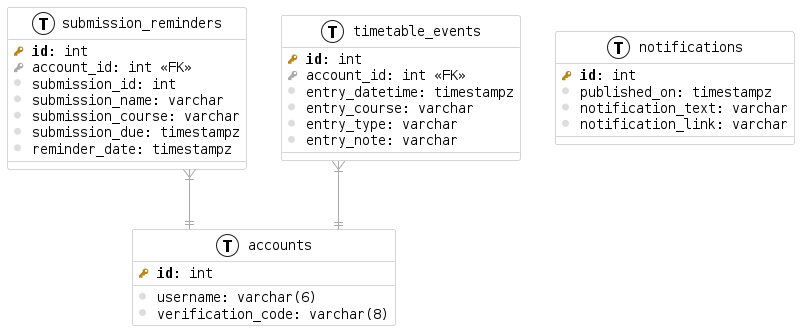
\includegraphics[width=\textwidth]{img/databazove-schema.png}
    \caption{Databázové schéma (vlastní zpracování)}\label{fig:db-schema}
\end{figure}
\imagesource{
@startuml
!define primary\_key(x) <b><color:#b8861b><&key></color> x</b>
!define foreign\_key(x) <color:#aaaaaa><&key></color> x
!define column(x) <color:#dddddd><&media-record></color> x

skinparam roundcorner 5
skinparam linetype ortho
skinparam defaultFontName Courier

skinparam class \{
    BackgroundColor white
    ArrowColor #aaaaaa
    BorderColor #aaaaaa
\}

entity accounts << (T,white) >> \{
  primary\_key( id ): int
  column( username ): varchar(6)
  column( verification\_code ): varchar(8)
\}

entity submission\_reminders << (T,white) >> \{
  primary\_key( id ): int
  foreign\_key( account\_id ): int <<FK>>
  column( submission\_id ): int
  column( submission\_name ): varchar
  column( submission\_course ): varchar
  column( submission\_due ): timestampz
  column( reminder\_date ): timestampz
\}

entity timetable\_events << (T,white) >> \{
  primary\_key( id ): int
  foreign\_key( account\_id ): int <<FK>>
  column( entry\_datetime ): timestampz
  column( entry\_course ): varchar
  column( entry\_type ): varchar
  column( entry\_note ): varchar
\}

entity notifications << (T,white) >> \{
  primary_key(id): int
  column(published\_on): timestampz
  column(notification\_text): varchar
  column(notification\_link): varchar
\}

submission\_reminders \}|--|| accounts
timetable\_events \}|--|| accounts
@enduml
}

\subsection{SQL migrace pomocí nástroje Liquibase}\label{chap:liquibase}

Pro jednodušší správu databázového schématu v rámci aplikace byl zvolen nástroj Liquibase. Jedná se o open source softwarové řešení pro správu verzí databázových schémat pomocí migrací definovaných v jednom z podporovaných datových formátů \cite{liquibase_inc_2023}.

Z podporovaných formátů, mezi které mimo jiné patří formát JSON, XML, YAML a SQL, byl zvolen pro potřeby podpůrného webového serveru formát SQL. Ten umožňuje definovat databázové migrace přímo v jazyce SQL rozšířeným o speciální kontrolní struktury chování, které je možné definovat jako komentáře. Všechny databázové migrace se nachází v souboru \code{/src/main/resources/changelog.sql}.


Ve výpise \ref{code:liquibase-changelog} se nachází 2 typy těchto speciálních komentářů, které slouží jako kontrolní struktury pro nástroj Liquibase. Prvním typem je komentář \code{-{}-liquibase formatted sql} na prvním řádku souboru. Tímto komentářem musí začínat všechny soubory, které se mají zpracovat nástrojem Liquibase. Jedná se především o kontrolní mechanismus, který zajišťuje, aby nedošlo k spouštění SQL souborů, které nejsou určeny pro zpracování nástrojem Liquibase a neobsahují komentáře pro kontroly a definice migrací. Druhým typem speciálního komentáře jsou definice jednotlivých migrací. Každá migrace je definována pomocí speciálního komentáře \code{-{}-changeset}, který je následován dvojicí argumentů spojených dvojtečkou. Prvním argumentem je autor migrace a druhým je unikátní identifikátor označující danou migraci \cite{liquibase_inc_sql_changelog}.

\subsection{Definice doménových tříd a repozitářů}

Modul Spring Data aplikačního rámce Spring umožňuje deklarativně mapovat data z databázových tabulek na atributy doménových tříd za pomocí anotací. Přikladem může být doménová třída \code{TimetableEvent}. Obsah souboru, ve kterém je tato třída definována je možné vidět ve výpise \ref{code:timetable-event-domain-class}. Mapování třídy na tabulku je realizováno pomocí anotace \code{@Table}, která jako parametr očekává název tabulky ze které se mají mapovat hodnoty. Další anotací, kterou modul Spring Data využívá pro mapování dat je anotace \code{@Id}, která indikuje, že anotovaný atribut odpovídá primárnímu klíči v mapované tabulce. Takto anotovaný atribut musí být v každé doménové třídě právě jeden. Tato anotace slouží mimo jiné i pro cachování a recyklaci vytvořených instancí, správy namapovaných entit a optimalizaci vygenerovaných databázových dotazů. Poslední anotací, které se v rámci zmíněné doménové třídy využívá pro definici mapování, je anotace \code{@Column}. Tato anotace očekává jako parametr název sloupce, který v databázové tabulce odpovídá anotovanému atributu definovaném v doménové třídě. Konverze datových typů probíhá automaticky a je zajištěna ovladačem pro konkrétní systém řízení báze dat.

Pro načítání a ukládání dat z tabulek pomocí doménových tříd slouží takzvané repozitáře. Při použití tradičního způsobu načítání dat z relačních databází v programovacím jazyce Java je zapotřebí ručně psát databázové SQL dotazy a zpracovávat výsledky dotazu pomocí tříd a rozhraní z balíčku \code{java.sql}. Tento přístup je velice pracný a náchylný na chyby, které můžou nastat například v podobě nevalidních SQL dotazů, nesprávné implementace mapování a konverze datových typů po načtení dat z databáze nebo v podobě chyb souvisejících s narušením referenční integrity. 

Aplikační rámec Spring a modul Spring Data umožňuje tento tradiční přístup, který by bylo možné onznačit za spíše imperativní, nahradit deklarativní definicí repozitářů, které se starají o načítání, cachování a ukládání dat pro konkrétní doménovou třídu a tedy posléze namapovanou databázovou tabulku. Nespornou výhodou repozitářů je jednoduchost jejich definice a použití. Repozitář lze definovat jako rozhraní označené anotací \code{@Repository}. Spring Data automaticky při vytváření aplikačního kontejneru vytvoří a zaregistruje instanci anonymní třídy, která implementuje definované rozhraní. Tuto instanci je možné následně z aplikačního kontejneru získat pomocí dependency injection. Spring Data automaticky derivuje SQL dotazy z názvu metod podle konvencí definovaných v referenční dokumentaci tohoto modulu. Spring Data poskytuje řadu již definovaných generických rozhraní pro repozitáře, ze kterých je možné pro konkrétní repozitář zdědit často využívané definice metod. Příkladem může být generické rozhraní \code{CoroutineCrudRepository<T, ID>}, které obsahuje sadu definovaných CRUD\footnote{Create, Read, Update, Delete} metod jako je například \code{findById(id: ID): T}, která podle jmenné konvence odpovídá SQL dotazu \code{SELECT * FROM :table WHERE id = :id}. Například metoda \code{findByIdAndAccount} definovaná na repozitáři \code{TimetableEventsRepository} vypsaném ve výpise \ref{code:timetable-events-repository} odpovídá podle jmenné konvence SQL dotazu \code{SELECT * FROM timetable\_events WHERE id = :id AND account\_id = :account} ve kterém se za parametry \code{:id} a \code{:account} dosadí hodnoty předané při volání této metody.

\todo{Ocitovat Spring Data dokumentaci ohledně derivace repozitářů?}

\section{Vrstva pro zajištění business logiky}

\subsection{Definice opakujících se událostí pro rozesílání upozornění}

Opakující se události je možné v rámci aplikačního rámce Spring definovat pomocí metod s anotací \code{@Scheduled}. Tato anotace přijímá kombinaci parametrů, které umožňují flexibilně sestavovat časové intervaly, ve kterých se má anotovaná metoda volat. Toho využívá třída \code{SendSubmissionRemindersNotificationsTask}, která obsahuje metodu \code{run}, kterou je možné vidět ve výpise \ref{code:send-submission-reminders-notifications-task}, která se spouští každých 5 minut. 

Tato metoda nejprve provede kontrolu, že aplikace není spuštěná v testovacím prostředí a následně zavolá metodu \code{sendPendingSubmissionRemindersNotifications} na injektované instanci třídy \code{SubmissionRemindersService}.

\begin{lstlisting}[label={code:send-submission-reminders-notifications-task}, caption={Definice periodicky spouštěné metody run}]
@Scheduled(
    fixedRate = 5,
    timeUnit = TimeUnit.MINUTES
)
fun run(): Unit = runBlocking {
    // Do not run this task during tests
    if (!environment.acceptsProfiles(Profiles.of("test"))) {
        service.sendPendingSubmissionRemindersNotifications()
    }
}
\end{lstlisting}

\section{Prezentační vrstva}

Prezenční vrstva slouží pro komunikaci s klienty API. To zahrnuje mimo jiné přijímání HTTP požadavků, validaci formátu a obsahu dat požadavku nebo odesílání HTTP odpovědí. Prezenční vrstva je tvořena ze dvou typů komponent, kontrolerů a rozhraní pro přenos a validaci dat.

\subsection{Definice tříd kontrolerů}

\todo{Popsat strukturu HTTP požadavků?}

Kontrolery jsou speciálním typem tříd anotovaných pomocí anotace \code{@Controller} nebo specializovaných variant jako například \code{RestController}, které se starají o odbavování HTTP požadavků. Každému HTTP endpointu, který příjimá požadavky odpovídá právě jedna metoda na kontroleru, která je označena anotací \code{RequestMapping} nebo některou z jejich specializovaných variant. Tyto varianty jsou vázány na konkrétní HTTP metody a příkladem těchto specializovaných variant může být například anotace \code{@GetMapping}, která odpovídá na HTTP požadavky využívající metodu \code{GET} \cite[kap. 1.3.1]{walls_spring_2019}.

Příkladem kompletní definice a implementace kontroleru je třída \code{AccountsController}, kterou je možné vidět ve výpise \ref{code:accounts-controller}. Aplikační rámec Spring automaticky registruje třídy anotované pomocí \code{@RestController}, protože tato anotace dědí logiku z anotace \code{@Component}, která způsobí vytvoření nové instance v rámci aplikačního kontejneru \cite[kap. 11.1.2]{walls_spring_2019}.

Argument anotace \code{@RequestMapping} definuje část URL adresy, která je společná pro všechny metody bez vazby na konkrétní HTTP metodu. Metoda \code{createAccount}, která je anotovaná pomocí anotace \code{@PostMapping} s parametrem \code{"/create"} bude tedy dostupná pomocí HTTP metody POST na URL adrese \code{/api/v1/account/create}. Druhá metoda \code{verifyAcocunt}, která je anotovaná pomocí anotace \code{@PostMapping} s parametrem \code{"/verify"} bude dostupná obdobně jako metoda \code{createAccount} pomocí HTTP metody POST, ale tentokrát na adrese \code{/api/v1/account/verify}.

Tyto metody, které slouží pro obsluhu HTTP požadavků mají jako návratový typ generickou třídu \code{ResponseEntity<T>}. Instance této třídy aplikační rámec Spring následně převádí na HTTP odpověďi, které odešle klientovi. Tento datový typ obsahuje informace o stavovém kódu, HTTP hlavičkách včetně hlavičky \code{Content-Type} a obsahu těla HTTP požadavku, jehož struktura odpovídá generickému typu \code{T} a který je následně serializován do formátu JSON. Tato serializace je důsledek použití anotace \code{RestController}, která oproti obecné anotaci \code{Controller} implikuje, že všechny výstupní hodnoty volání obslužných metod mají být serializovány a odeslány s patřičnou hlavičkou \code{Content-Type}, jejíž hodnota je automaticky nastavena na hodnotu \code{application/json}.

\subsection{Definice tříd pro přenos dat}

Pro jasné vymezení datových typů reprezentující požadavky, které aplikace v metodách kontrolerů přijímá, se využívají takzvané DTO\footnote{Data Transfer Object} třídy. Tento typ tříd se používá pro definici struktury požadavku nebo odpovědi společně s validačními pravidly, které aplikační rámec Spring před zavoláním metody kontroleru validuje. Jednou z takových tříd je například třída \code{CreateAccountRequest}, jejíž definici je možné vidět ve výpise \ref{code:create-account-request}, a kterou jako vstupní parametr očekává již zmíněná metoda \code{createAccount}. Tento parametr je anotovaný pomocí anotace \code{@RequestBody}, která dává aplikačnímu rámci Spring instrukci, že se mají hodnoty definované v této třídě načíst z těla HTTP požadavku, a dále pomocí anotace \code{@Valid}, která implikuje validaci požadavku pomocí pravidel definovaných na jednotlivých atributech třídy \code{CreateAccountRequest}.

Třída \code{CreateAccountRequest} obsahuje jediný atribut s názvem \code{username}, na kterém jsou pomocí anotací z balíčku \url{jakarta.validation.contraints} definované 3 pravidla, které se musí před voláním zvalidovat. Anotace \code{@NotBlank} určuje, že tento parametr nesmí v požadavku chybět a že se nemůže jednat o prázdný textový řetězec nebo o textový řetězec, který je tvořený pouze z netisknutelných znaků. Dále anotace \code{@Size} definuje pomocí parametrů \code{min} a \code{max} minimální a maximální délku textového řetězce tohoto atributu. Poslední anotací, která definuje validační pravidla pro atribut \code{username} je anotace \code{@Pattern}, která pomocí parametru \code{regexp} definuje regulární výraz, který se musí shodovat s hodnotou v atributu \cite[kap 2.3]{walls_spring_2019}. Tento konkrétní regulární výraz odpovídá formátu emailových adres přidělovaných studentům na Vysoké škole ekonomické v Praze. Ve výpise je možné si všimnout, že všechny takto aplikované anotace začínají výrazem \code{field:}. Tato syntaxe v jazyce Kotlin udává, na kterou z částí vygenerovaného JVM kódu se má anotace aplikovat. V případě \code{field} se anotace umístí na vygenerovanou statickou instanční proměnnou v rámci syntetizované třídy \cite{ebel_mastering_2019}.

\section{Testování}\label{sec:testovani}

Testování je proces pro zajištění kvality vyvíjeného softwarového řešení. Testování se dělí na dvě hlavní části. Prvním typem je uživatelské testování, které se často označuje také jako manuální testování. V tomto typu testování probíhá kontrola implementace pomocí ručního spouštění funkcionalit dle předem stanovených scénářů. Druhým typem je strojové testování, kdy testování probíhá pomocí spouštění testovacího kódu, který ověřuje správnou funkčnost testovaného kódu. Oba typy testování mají řadu výhod a nevýhod oproti druhému typu. Výhodou uživatelského testování je lidský faktor, který je v procesu zahrnut. Tento lidský faktor umožňuje detekovat řádu kódovacích chyb, které nejsou možné pomocí strojových testů odhalit. Další výhodou manuálního testování je, že testovaný scénář přímo odpovídá zkušenosti uživatele koncového softwarového produktu a testování často probíhá na reálných zařízeních, které se mohou chovat odlišně, pokud se jedná o simulátor. Uživatelské testování se často využívá při testování UI a UX aspektů softwarového řešení. Největší nevýhodou manuálního testování oproti strojovému je jeho časová a finanční náročnost společně s velice omezenou možností replikace. Strojové testy je možné spouštět paralelně, zatímco tester musí uživatelské testy provádět sekvenčně. Kromě rychlosti spouštění testů v případě strojového testování je výhodou snadná replikace. Sadu strojových testů je možné bez větších nákladů spouštět iterativně po každé změně a je možné takto kontinuálně ověřovat korektnost implementace. Oproti tomu, v případě uživatelského testování je potřeba předat kód s testovacím prostředím testerovi a a počkat na zpracování testovacích scénářů, které v případě většiho množství scénářů může trvat i několik hodin. Další výhodou strojových testů je možnost jejich integrace jako součást nasazení kódu v rámci systému pro správu verzí kódu. V takovém případě je možné zařadit spouštění strojových testů do pipeline, která probíhá například před každou změnou hlavní vývojové větve pro zajištění integrity a minimalizace chyb v produkčním prostředí.

Strojové testy je možné dále dělit podle jejich granuality, tedy jak širokou část výsledného systému testují. Testy s největší granualitou se označují jako takzvané jednotkové testy\footnote{Často se používá také anglický termín unit test} pipeline. Tyto jednotkové testy se vymezují na jednotku kódu, často se jedná o konkrétní metodu nebo třídu. Tento typ testů je vhodný zejména pro testování implementace algoritmů a zajištění shody implementace se specifikací. Těchto testů je oproti ostatním typům strojových testů velké množství a velice často je možné jejich spouštění paralelizovat, protože testují izolované části systému. Dalším typem strojových testů jsou takzvané integrační testy, které se zaměřují již na větší část systému, ve které dochází ke spojení několika menších jednotek, které jsou samostatně testovány pomocí testů jednotkových. 

\todo{Dopsat integrační testy a akceptační testy, zdroje}

\subsection{Strojové testy JUnit a jejich podpora v aplikačním rámci Spring}

Zdaleka nejpopulárnějším nástrojem pro psaní strojových testů v programovacích jazycích platformy JVM je testovací framework JUnit. Tento framework umožňuje spouštění definovat a spouštět testy pomocí anotací nad metodami testovacích tříd. Kromě řídících anotací jako je anotace \code{@Test}, která označuje metodu s testovacím kódem poskytuje framework JUnit rozhraní pro definici takzvaných assertion výrazů, které ověřují vlastnosti zadaných parametrů. Nejčastějším příkladem takového assertion výrazu je metoda \code{Assertions.assertEquals(} \code{expected, actual)}, která kontroluje, že parametry \code{expected} a \code{actual} nabývají stejné hodnoty. Dalšími takovéto metody mohou být například metody \code{assertNotNull}, \code{assertTrue}, \code{assertThrows} nebo \code{assertLinesMatch}. Pokud předaný parametr nevyhovuje výrazu, který ověřuje některou z jeho vlastností, dojde v rámci testovacího frameworku k vyvolání výjimky, která je testovacím rámcem odchycena a která způsobí, že daný test je označen za neúspěch. Pokud předaný parametr testovaným podmínkám vyhovuje, test pokračuje až do vykonání poslední instrukce v rámci testovací metody. Pokud celá testovací metoda označená anotací \code{@Test} proběhne až do konce bez vyvolání výjimky, je test označen jako úspěch \cite{gulati_junit_2017}

Aplikační rámec Spring zjednodušuje psaní JUnit testů pomocí přidaných anotací, jako je například \code{SpringBootTest}, které před spuštěním testů umožňují nakonfigurovat aplikační kontejner se všemi potřebnými závislostmi. Dále poskytuje celou řadu nástrojů sloužících pro testování konkrétních aspektů využívaných v rámci aplikace. Přikladem může být testovací třída \code{WebTestClient}, která umožňuje simulovat odesílání HTTP požadavků a obsahuje aplikační rozhraní pro validaci HTTP odpovědí na tyto požadavky. Mezi tyto validace patří mimo jiné validace stavového kódu HTTP odpovědi, obsahu a prezence HTTP hlaviček nebo validace hodnot ve zparsovaném tělu HTTP odpovědi, které je nejčastěji buď ve formátu JSON nebo ve formátu XML.

\subsection{Testcontainers}

Častým problémem při spouštění integračních testů je zajištění komunikace s databází nebo jinými externími službami, které jsou závislostmi některých částí aplikace. Tento problém řeší nástroj Testcontainers, který umožňuje strojově spouštět pomocí nástroje Docker kontejnery s instancemi těchto externích služeb a zároveň je automaticky registrovat do aplikačního kontextu. Tento nástroj má oficiální podporu pro širokou škálu technologií, které mimo jiné zahrnují programovací jazyky Java, Go, Python, JavaScript nebo Haskell.

Jedinou externí službou využívanou v rámci podpůrného webového serveru je systém pro řízení báze dat PostgreSQL, pro který je možné v aplikačním rámci Spring vytvářet při spouštění integračních testů instance skrze kombinaci balíčků \code{org.testcontainers:postgresql} a \code{org.testcontainers:r2dbc}, které poskytují R2DBC-kompatibiliní ovladače pro PostgreSQL. Po instalaci balíčků je možné nakonfigurovat databázové připojení pro spouštění integračních testů v souboru \code{application-test.yml}, který zobrazuje výpis \ref{code:application-test-yml}.

V nástroji Testcontainers dochází ke specifikaci běhového prostředí přes atributy v URL připojení. Tato specifikace může zahrnovat například verzi docker image, která se má před spuštěním testů instanciovat. Technologie Docker je dále popsaná v sekci \ref{sec:docker}.

\begin{lstlisting}[label={code:application-test-yml}, caption={Konfigurace prostředí pro spouštění testů s využitím testcontainers (vlastní zpracování)}]
spring:
  datasource:
    url: jdbc:tc:postgresql:13.9:///vse-plus-api
    username: vse-plus-api
    password: vse-plus-api
    driver-class-name: org.testcontainers.jdbc.ContainerDatabaseDriver
  liquibase:
    url: ${spring.datasource.url}
    user: ${spring.datasource.username}
    password: ${spring.datasource.password}
    driver-class-name: ${spring.datasource.driver-class-name}
  r2dbc:
    url: r2dbc:tc:postgresql:///vse-plus-api?TC_IMAGE_TAG=13.9
    user: ${spring.datasource.username}
    password: ${spring.datasource.password}
  mail:
    host: smtp.mailtrap.io
    port: 25
    username: username
    password: password
    test-connection: false
 
\end{lstlisting}

\subsection{Automatické spouštění testů pomocí GitLab CI/CD}

Jak již bylo zmíněno v sekci \ref{sec:testovani}, spouštění strojových testů je často součástí integračních pipeline, které jsou spouštěny jako součá CI/CD pipeline, jejíž definice je možné vidět ve výpise \ref{code:gitlab-ci-docker}. Této praktiky využívá i projekt s kódem podpůrného serveru hostovaný na platformě GitLab, kde probíhá automatické spouštění testů pomocí vestavěného nástroje GitLab CI/CD při integraci každé nové změny. Tyto testy jsou pak v rámci úlohy na CI serveru vyexportovány jako pipeline artefakty a je možné si zobrazit výsledky spouštění testů přímo v platformě GitLab jak zobrazuje obrázek \ref{fig:gitlab-ci-junit} \cite{gitlab_unit_test_reports}. 

\begin{figure}[htbp!]\centering
    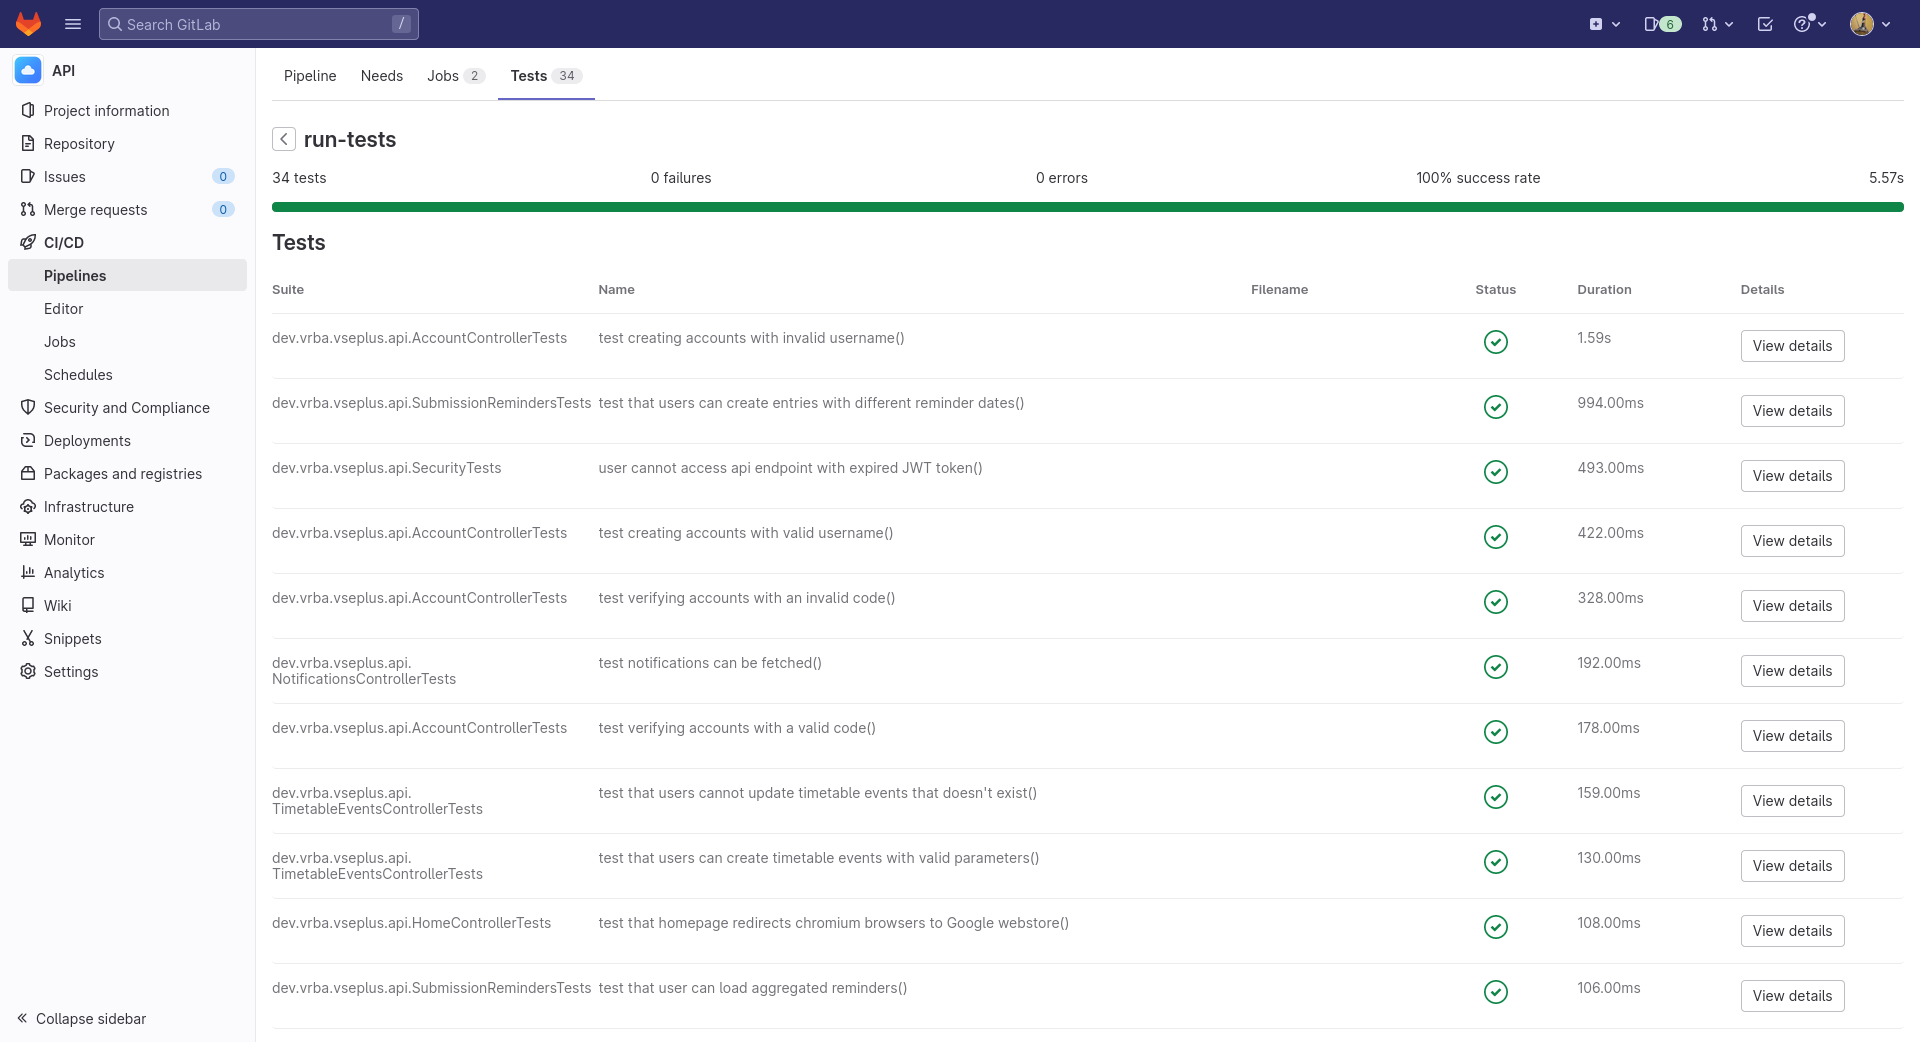
\includegraphics[width=\textwidth]{img/gitlab-ci-junit.png}
    \caption{Výsledky spuštění JUnit testů v platformě GitLab (vlastní zpracování)}
    \label{fig:gitlab-ci-junit}
\end{figure}
 
\section{Nasazení aplikace}

Pro nasazení podpůrného serveru je potřeba zvážit hned několik faktorů, které hrají roli. 
Prvním z těchto faktorů je otázka jak bude probíhat distribuce softwaru, tj. jak se bude sestavovat aplikační balíček a jak se bude tento aplikační balíček spouštět. 
Dalším faktorem pro zvážení před nasazením aplikace je provozní cena. Jelikož se jedná o dlouhodobě běžící projekt s~nulovou návratností a protože rozšíření je poskytováno zcela zdarma, byla vyvinuta snaha snížit náklady spojené s~provozem aplikace na minimum.

\subsection{Výběr hostingu}

\todo{Srovnání platform pro hostování docker containerů, výběr DO}

\subsection{Využítí technologie Docker}\label{sec:docker}

Docker je technologie pro virtualizaci a izolaci běhového prostředí aplikací za pomocí takzvaných kontejnerů. Tyto kontejnery jsou alternativou k tradičním enterprise nástrojům pro virtualizaci jako například VMware nebo KVM. Kontejnery se od virtuálních počítačů liší tím, že s hostujícím operačním systémem sdílí systémové jádro\footnote{V angličtině se pro označení jádra označuje termín system kernel} a jsou tedy mnohem méně náročné na systémové prostředky pro chod virtualizovaného systému, protože nedochází k simulaci hardwarových prostředků a operačního systému s překladem systémových volání \cite[kap. 1]{kane_docker_2018}.

Docker umožňuje snadno vytvářet, spravovat a sdílet tyto kontejnery, což výrazně usnadňuje proces distribuce softwarových balíčků a jejich závislostí, protože je možné celou aplikace včetně všech závislostí zabalit do připraveného kontejneru s nakonfigurovaným běhovým prostředím. 

Docker pracuje s konceptem takzvaných images, které si lze představit jako šablonu pro vytváření kontejnerů. Tyto image jsou projekcí stavu souborového systému a z jedné image je možné vytvořit neomezené množství kontejnerů, které pak následně nástroj docker spravuje. 

\todo{srovnání tradičního deploymentu s dockerem?}

\subsection{Automatické sestavování docker image pomocí GitLab CI/CD}

Pro sestavení docker image obsahující zdrojové kódy a běhové prostředí pro podpůrný webový server je možné využít kombinaci nástrojů GitLab CI/CD a GitLab Container Registry. GitLab Container Registry je platforma implementující protokol pro vytváření a publikaci repozitářů pro docker image.

\todo{Odkaz na GitLab repozitář https://gitlab.com/vse-plus/api}